\section{Tổng quan Hệ thống (System Overview)}
\label{sec:tong-quan}

Phần này cung cấp một cái nhìn tổng quan về dự án ở mức cao nhất, trả lời các câu hỏi cơ bản: "Dự án này giải quyết vấn đề gì?", "Nó được xây dựng dựa trên kiến trúc nào?", và "Luồng dữ liệu cốt lõi hoạt động ra sao?".

\subsection{Mục tiêu Kinh doanh}
\label{subsec:muc-tieu-kinh-doanh}

Mục tiêu cốt lõi của dự án là xây dựng và vận hành một nền tảng Phần mềm dưới dạng Dịch vụ (SaaS - Software as a Service) chuyên biệt, cung cấp một giải pháp Live Chat hiện đại và mạnh mẽ cho các chủ sở hữu website. 

Sản phẩm được thiết kế để có thể dễ dàng tích hợp vào bất kỳ website nào thông qua một đoạn mã JavaScript (widget) đơn giản. Chức năng chính của widget này là tạo ra một kênh giao tiếp trực tiếp, tức thời giữa doanh nghiệp và khách truy cập (visitor) ngay trên trang web của họ, mà không cần chuyển hướng qua các ứng dụng nhắn tin của bên thứ ba.

Điểm khác biệt và là giá trị cốt lõi mà sản phẩm mang lại không chỉ dừng lại ở việc trò chuyện, mà còn cung cấp những "siêu năng lực" cho nhân viên hỗ trợ. Bằng cách thu thập và hiển thị các dữ liệu ngữ cảnh quan trọng theo thời gian thực (ví dụ: khách truy cập đang xem chính xác trang sản phẩm nào, lịch sử duyệt web của họ trên trang), nền tảng của chúng ta cho phép các nhân viên hỗ trợ bắt đầu một cuộc hội thoại một cách thấu hiểu và cá nhân hóa, từ đó tăng cường khả năng chuyển đổi, cải thiện sự hài lòng của khách hàng và xây dựng mối quan hệ bền vững.
\subsection{Mô hình Kiến trúc}
\label{subsec:mo-hinh-kien-truc}

Kiến trúc tổng thể của hệ thống được xây dựng theo mô hình \textbf{Modular Monolith} (Khối đơnolithic dạng Module), vận hành trên nền tảng \textbf{NestJS} (sử dụng TypeScript).

Lựa chọn kiến trúc này mang lại sự cân bằng chiến lược: vừa có được tốc độ phát triển nhanh và sự đơn giản trong việc triển khai của một ứng dụng Monolith, vừa duy trì được cấu trúc ranh giới rõ ràng giữa các domain nghiệp vụ khác nhau (như User, Project, Inbox...). Cấu trúc module hóa này không chỉ giúp codebase có tổ chức và dễ bảo trì, mà còn là một bước đệm quan trọng, cho phép hệ thống có thể được tách ra thành các Microservices riêng biệt trong tương lai một cách thuận lợi khi quy mô phát triển.

Tuy nhiên, kiến trúc này không hoàn toàn đồng bộ. Để đảm bảo độ tin cậy và khả năng mở rộng cho các tác vụ quan trọng, hệ thống đã tích hợp thêm các thành phần bất đồng bộ:
\begin{itemize}
    \item \textbf{AWS Simple Queue Service (SQS):} Được sử dụng làm hàng đợi tin nhắn (message queue) cho luồng xử lý sự kiện chính. Khi một tin nhắn từ visitor được gửi đến, nó sẽ được đẩy vào SQS ngay lập tức. Một tiến trình Worker riêng biệt sẽ lấy tin nhắn từ hàng đợi để xử lý logic nghiệp vụ. Kiến trúc Producer-Consumer này giúp tách biệt lớp giao tiếp real-time khỏi lớp xử lý nghiệp vụ, đảm bảo hệ thống không bao giờ làm mất tin nhắn và có khả năng chống chịu khi lưu lượng truy cập tăng đột biến.
    
    \item \textbf{Redis:} Đóng hai vai trò quan trọng trong hệ thống:
    \begin{enumerate}
        
        \item 
        \begin{sloppypar}
            \textbf{WebSocket Backplane:} Thông qua \texttt{RedisIoAdapter}, Redis hoạt động như một lớp nền giao tiếp (backplane), cho phép nhiều server instance của WebSocket Gateway có thể giao tiếp và chia sẻ trạng thái với nhau. Đây là yếu tố then chốt cho phép lớp real-time có thể mở rộng theo chiều ngang (horizontal scaling).
        \end{sloppypar}

        \item \textbf{Quản lý Session:} Redis được sử dụng để lưu trữ và tra cứu trạng thái kết nối (session) của các visitor. Nó ánh xạ định danh của visitor (\texttt{visitorUid}) với ID kết nối socket (\texttt{socket.id}) của họ, giúp hệ thống có thể gửi tin nhắn đến đúng người nhận một cách nhanh chóng và hiệu quả.
    \end{enumerate}
\end{itemize}
\subsection{Luồng Dữ liệu Cốt lõi}
\label{subsec:luong-du-lieu-cot-loi}

Để hiểu rõ cách các thành phần kiến trúc phối hợp với nhau, phần này sẽ mô tả và sơ đồ hóa hai luồng dữ liệu quan trọng nhất của hệ thống: luồng tin nhắn từ khách truy cập (visitor) đến nhân viên hỗ trợ (agent), và luồng tin nhắn trả lời theo chiều ngược lại.

\subsubsection{Luồng 1: Tin nhắn từ Visitor đến Agent}

Đây là luồng xử lý bất đồng bộ, được thiết kế để đảm bảo độ tin cậy và khả năng mở rộng.

\begin{enumerate}
    \item \textbf{Gửi tin nhắn:} Khách truy cập gõ và gửi một tin nhắn từ Chat Widget trên website.
    \item \textbf{Tiếp nhận Real-time:} Widget gửi sự kiện \texttt{sendMessage} qua kết nối WebSocket (WSS) đến \textbf{WebSocket Gateway}.
    \item \textbf{Đưa vào hàng đợi:} Gateway tiếp nhận sự kiện, đóng gói payload và ngay lập tức đẩy nó vào hàng đợi \textbf{AWS SQS}. Gateway không thực hiện bất kỳ xử lý nghiệp vụ nào.
    \item \textbf{Xử lý bất đồng bộ:} Một tiến trình \textbf{Event Consumer Worker} độc lập lắng nghe và nhận tin nhắn từ hàng đợi SQS.
    \item 
    \begin{sloppypar}
        \textbf{Lưu trữ dữ liệu:} Worker thực thi logic nghiệp vụ (tìm hoặc tạo visitor, conversation) và lưu tin nhắn mới vào \textbf{Database}.
    \end{sloppypar}
    \item \textbf{Thông báo cho Agent:} Sau khi lưu thành công, Worker phát một sự kiện nội bộ (thông qua Redis Pub/Sub) để thông báo cho Gateway rằng có tin nhắn mới.
    \item \textbf{Cập nhật Dashboard:} Gateway nhận sự kiện nội bộ và phát sự kiện \texttt{newMessage} đến Dashboard của các Agent đang theo dõi dự án tương ứng.
\end{enumerate}

\subsubsection{Luồng 2: Tin nhắn trả lời từ Agent đến Visitor}

Đây là luồng xử lý đồng bộ hơn, tập trung vào việc gửi tin nhắn đến đúng người nhận một cách nhanh chóng.

\begin{enumerate}
    \item \textbf{Gửi trả lời:} Nhân viên hỗ trợ gõ và gửi tin nhắn trả lời từ Agent Dashboard.
    \item \textbf{Yêu cầu HTTP:} Dashboard gửi một request \texttt{POST} đến \textbf{Backend API} (ví dụ: \texttt{/api/v1/inbox/conversations/:id/messages}).
    \item \textbf{Lưu trữ dữ liệu:} Backend API xác thực quyền của agent và lưu tin nhắn trả lời vào \textbf{Database}.
    \item \textbf{Tra cứu Session:} Backend API gọi đến \textbf{RealtimeSessionService} để tra cứu \texttt{socket.id} hiện tại của visitor từ \textbf{Redis}, dựa trên \texttt{visitorUid} của cuộc hội thoại.
    \item \textbf{Yêu cầu gửi Real-time:} Nếu visitor đang online (tìm thấy \texttt{socket.id}), Backend API sẽ yêu cầu \textbf{WebSocket Gateway} gửi tin nhắn đi.
    \item \textbf{Gửi tin nhắn:} Gateway gửi sự kiện \texttt{agentReply} trực tiếp đến \texttt{socket.id} của visitor, đảm bảo chỉ người nhận chính xác mới thấy được tin nhắn.
\end{enumerate}

\subsubsection{Sơ đồ Chuỗi tương tác (Sequence Diagram)}

Sơ đồ dưới đây trực quan hóa cả hai luồng dữ liệu đã mô tả ở trên.

\begin{figure}[h!]
    \centering
    \caption{Sơ đồ Luồng dữ liệu Tin nhắn}
    \label{fig:sequence-diagram}
    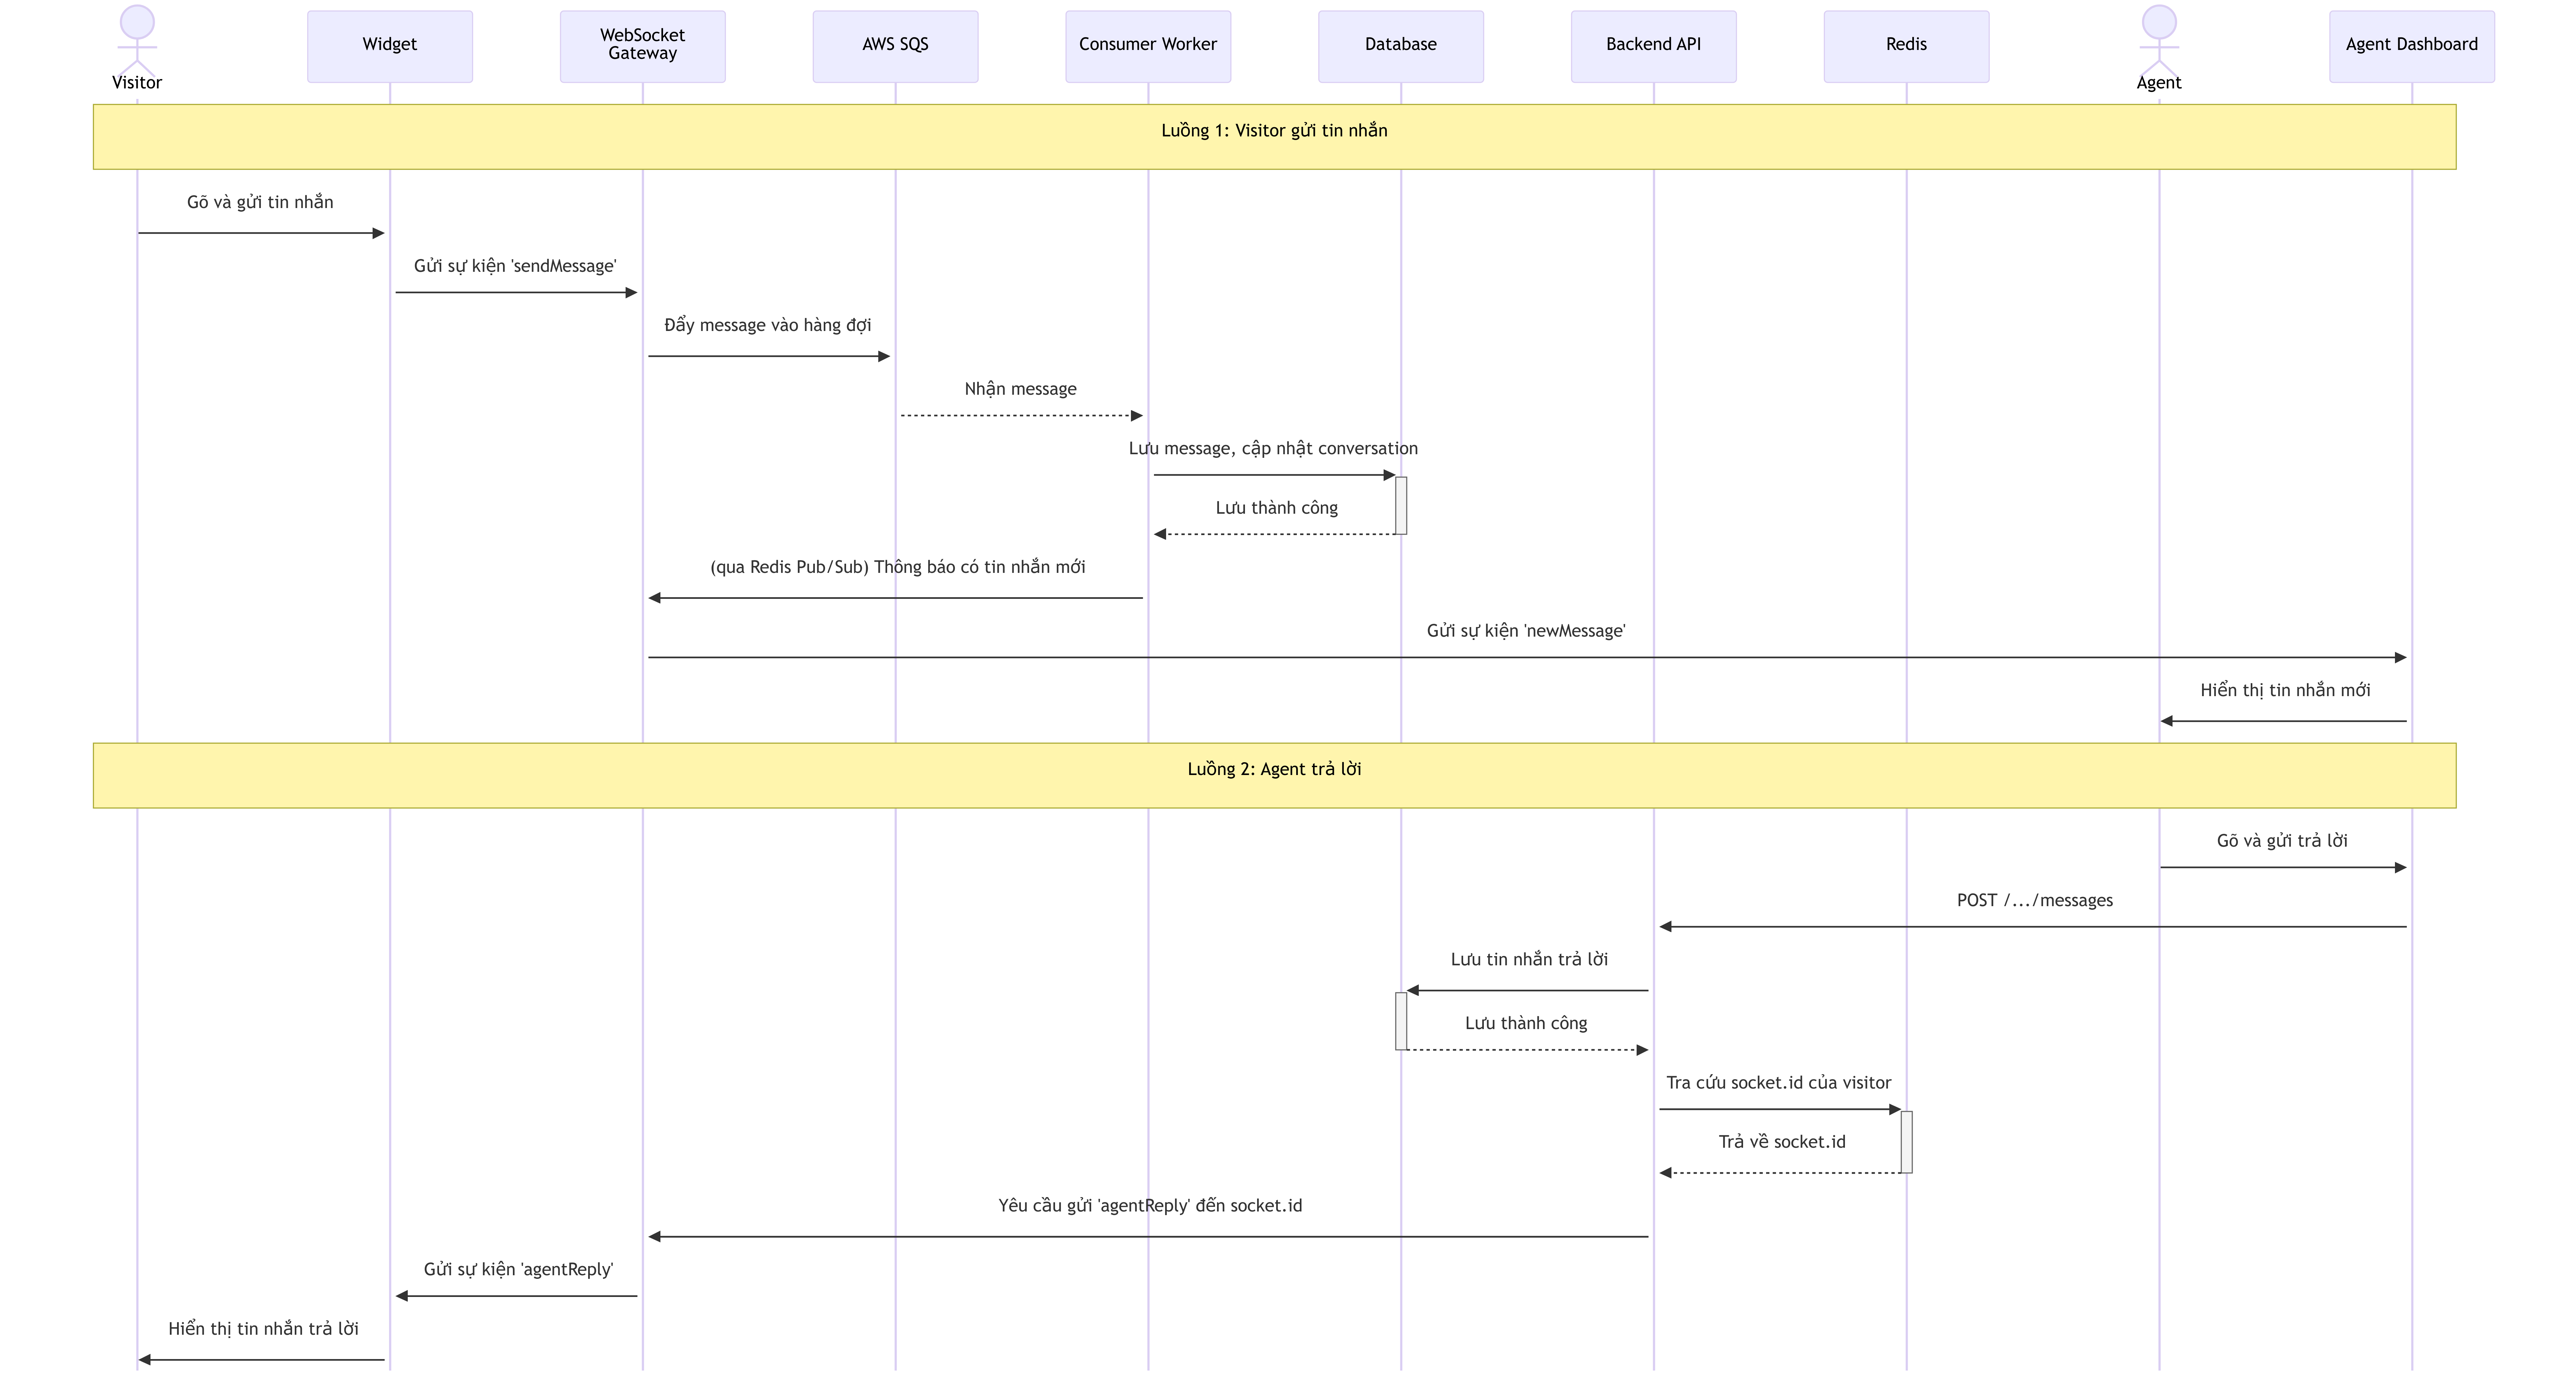
\includegraphics[width=1\textwidth]{images/inbox-diagram.png}
\end{figure}